\documentclass{article}

\usepackage{aligned-overset}
\usepackage{amsmath}
\usepackage{amssymb}
\usepackage[shortlabels]{enumitem}
\usepackage{genealogytree}
\usepackage{hyperref}
\usepackage[utf8]{inputenc}
\usepackage{mathtools}
\usepackage{physics}
\usepackage{tikz}
\usetikzlibrary{positioning}
\usepackage{xcolor}
\definecolor{light-gray}{gray}{.9}

\author{Karsten Lehmann}
\date{WiSe 2020}
\title{Übung Analysis - Grundlegende Konzepte (AN10)}

\begin{document}


\maketitle

\vfill
\begin{center}
  Dozent: Hans-Peter Scheffler \\
  \href{mailto:hans-peter.scheffler@tu-dresden.de}{hans-peter.acheffler@tu-dresden.de}
\end{center}

\newpage

\section*{Übungsblatt 2}

\begin{itemize}
\item $(\mathbb{R}, +, *)$ ist ein Körper
\item A1 - A9
\item Ordnungsaxiome \\
  Es existiert eine nicht-leere Teilmenge $P \subseteq \mathbb{R}$
  \begin{enumerate}[label=(A\arabic*)]
    \setcounter{enumi}{9}
  \item $\forall a \in \mathbb{R} \colon a \in P \lor -a \in P \lor a = 0$
  \item $\forall a,b \in P \colon a + b \in P$
  \item $\forall a,b \in P \colon a * b \in P$
  \end{enumerate}
\end{itemize}

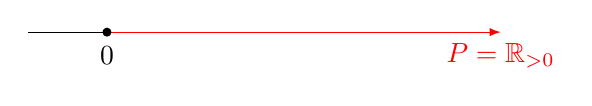
\begin{tikzpicture}
  \draw (0,0) -- (1,0);
  \draw[-latex, red] (1,0) -> (6,0);
  \node[draw, circle, fill, inner sep=1pt,  label=below:0] at (1,0) {};
  \node[red] at (6,-.3) {$P = \mathbb{R}_{>0}$};
\end{tikzpicture}

o$\leq$ ist eine reflexive Relation
\[
  \forall a \in \mathbb{R} \colon a \leq a
\]

\subsection*{Aufgabe 1}

\begin{enumerate}[(a)]
\item $\forall a,b,c \in \mathbb{R} \colon a < b \land b < c \Rightarrow a < c$ \\
  \begin{align*}
    (a < b) \land (b < c) &\iff (b - a \in \mathbb{R}_{>0}) \land (c - b \in \mathbb{R}_{>0}) \\
    \Rightarrow \mathbb{R}_{>0} \ni (b - a) + (c - b) \overset{\text{(A1), (A4)}}&{=} (c - a) + (b - b) \\
                                                      \overset{\text{(A3), (A2)}}&{=} c - a \\
                                                      & \Rightarrow c - a \in \mathbb{R}_{>0} \\
                                                      & \Rightarrow a < c\\
  \end{align*}
\item $\forall a,b,c \in \mathbb{R} \colon a < b \Rightarrow a + c < b + c$ \\
  \begin{align*}
    \mathbb{R}_{>0} \ni b - a \overset{\text{(A2)}}&{=} (b - a) + 0 \\
                              \overset{\text{(A3)}}&{=} (b - a) + (c - c) \\ 
                              \overset{\text{(A3), (A4), (A1)}}&{=} (b + c) - (a + c) \\
                              &\Rightarrow= b + c > a + c \\
  \end{align*}
\item $\forall a,b,c \in \mathbb{R} \colon 0 < a < b \Rightarrow 0 < b^{-1} < a^{-1}$ \\
  \begin{itemize}
  \item $a > 0 \Rightarrow a^{-1} > 0$:\\
    \textbf{Widerspruchsbeweis} \\
    Angenommen es gilt $a^{-1} < 0$. Dann ist $-a^{-1} > 0$, mittels (A12) und (A13)
    \[
      \overset{\text{(A12)}}\Rightarrow 0 < a * (-a^{-1}) = -(a * a^{-1}) \overset{\text{(A7)}}= -1 \\
    \]
    Dass heißt, es gilt $-1 > 0$, bzw. $-1 + 1 > 0$, dass heißt $0 > 1 \overset{\text{A6}}= 1 * 1 = 1^2$.
    Das ist ein Widerspruch zu $a^2 > 0$ für $a \ne 0$.
    Damit ist die Annahme $a^{-1} < 0$ falsch. Da $a^{-1} = 0$ schon ausgeschlossen wurde, gilt $a^{-1} > 0$.  
  \item $a < b \iff 0 < (b - a)$ \\
    Nun ist nach dem eben bewiesenen auch $a^{-1}b^{-1} > 0$
    \begin{align*}
      \overset{\text{(A12)}}\Rightarrow a^{-1} * b^{-1} > 0 \overset{\text{(A12)}}&\Rightarrow a(b - a) * (a^{-1}b^{-1}) \\
      \overset{\text{(A9)}}&{=} b * (a^{-1} * b^{-1}) -  a * (a^{-1} * b^{-1}) \\
      \overset{\text{(A5), (A8)}}&{=} a^{-1} * (b * b^{-1}) -  b^{-1} * (a * a^{-1}) \\
      \overset{\text{(A7), (A6)}}&{=} a^{-1} - b^{-1} \\
    \end{align*}
    Das heißt, $0 < a^{-1} - b^{-1}$ bzw. $0 < b^{-1} < a^{-1}$
  \end{itemize}
\end{enumerate}
\subsection*{Aufgabe2}
Für alle $a,b \in \mathbb{R}$ gilt
\[
  \text{max}\{a,b\} = \frac{1}{2}(a + b + \abs{a - b})
\]

Betrag für$a \in \mathbb{R} \colon \abs{a} = \begin{cases}
  a & a\geq 0 \\
  -a & a < 0 \\
\end{cases}
$

\begin{minipage}{.45\textwidth}
  \textbf{Fall 1:} \\
  Für $a \geq b$ gilt $\text{max}\{a,b\} = a$. Weiter ist $a - b > 0$, woraus folgt
  \begin{align*}
    \frac{1}{2}&(a + b + |a - b|) \\
               &= \frac{1}{2}(a + b + (a - b)) \\
               &= \frac{2}{2} a = a \\
               &= \text{max}\{a,b\} \\
  \end{align*}
\end{minipage}
\hfill
\vrule
\hfill
\begin{minipage}{.45\textwidth}
  \textbf{Fall 2:} \\
  Für $a < b$ gilt gilt $\text{max}\{a,b\} = b$. Weiter ist $a - b < 0$, woraus folgt
  \begin{align*}
    \frac{1}{2}&(a + b + |a - b|) \\
               &= \frac{1}{2}(a + b - (a - b)) \\
               &= \frac{2}{2} b = b \\
               &= \text{max}\{a,b\} \\
  \end{align*}
\end{minipage}

\subsection*{Aufgabe3}

\begin{enumerate}[a)]
\item
  \[
    L = \{ x \in \mathbb{R} | \abs{2x + 1} > x + 2\}
  \]

  \begin{minipage}{.4\textwidth}
    \textbf{Fall 1:} \\
    \begin{align*}
      2x &+ 1 > 0 \land |2x+1|\\
         &= 2x+1 > x+2 \\
         &\iff x \geq -\frac{1}{2} \land x > -3 \\
         &\iff x \in L1 \\
         &= \{ x \in \mathbb{R} | x \geq -\frac{1}{2} \} \\
         &= [-\frac{1}{2}, \infty) \\
    \end{align*}
  \end{minipage}
  \hfill
  \vrule
  \hfill
  \begin{minipage}{.4\textwidth}
    \textbf{Fall 2:} \\
    \begin{align*}
      2x &+ 1 < 0 \land |2x  + 1| \\
         &= -(2x + 1) > x - 2 \\
         &\iff x \geq -\frac{1}{2} \land x > -3 \\
         &\iff x \in L1 \\
         &= \{ x \in \mathbb{R} | x \geq -\frac{1}{2} \} \\
         &= [-\frac{1}{2}, \infty) \\
    \end{align*}
  \end{minipage}
\item
  \[
    L = \{ x \in \mathbb{R\abs{2x + 1}} > \abs{x - 2} \}
  \]
\item
  \[
    L = \{ x \in \mathbb{R} | \frac{x-7}{x-3} \leq x + 3 \}
  \]

\item
  \[
    L = \{ x \in \mathbb{R} | \frac{x - 7}{x - 3} > \frac{x + 3}{x + 5} \}
  \]

\end{enumerate}

Sei $A \subseteq \mathbb{R}, A \ne \emptyset$ $A$ is nach oben beschränkt: $\exists s \in \mathbb{R} \colon \forall a \in \mathbb{R} \colon a \leq s$ -> $s$ heißt obere Schranke von $A$


Ist $s$ eine obere Schranke von $M$, so ist auch jedes $s' > s$ eine obere Schranke von $M$. $s$ heißt Supremum von
$M$ wenn gilt:
\begin{enumerate}
\item $s$ ist obere Schranke
\item Ist $s'$ eine obere Schranke von $M$, so gilt $s' \geq s$
\end{enumerate}

=> $s$ ist die kleinste obere Schranke

Ist $M$ nach oben unbeschränkt ist, so wird das  $sup A \coloneq \infty$

\subsection*{Aufgabe 6}
\begin{enumerate}[(a)]
\item
  \begin{align*}
    A &= \{ n \in \mathbb{N} | n \text{ ist Teiler von } 24\} \\
      &= \{ 1,2,3,4,6,8,12,24 \}
  \end{align*}
\item
\begin{align*}
    A &= \{ n \in \mathbb{N} | n \text{ ist Teiler von } 24\} \\
      &= \{ 1,2,3,4,6,8,12,24 \}
  \end{align*}  
\end{enumerate}
\end{document}
